\documentclass{report}
\usepackage{graphicx, tikz-cd, float, titlepic, booktabs} % Required for inserting images
\usepackage{pgfplots}
\pgfplotsset{compat=1.15}
\usepackage{mathrsfs}
\usetikzlibrary{arrows}
\usepackage{amsmath, amssymb, amsthm, amsfonts, siunitx, physics, gensymb}
\AtBeginDocument{\RenewCommandCopy\qty\SI}
\usepackage[version=4]{mhchem}
\usepackage[most,many,breakable]{tcolorbox}
\usepackage{xcolor, fancyhdr, varwidth}
\usepackage[Glenn]{fncychap}
%Options: Sonny, Lenny, Glenn, Conny, Rejne, Bjarne, Bjornstrup
\usepackage{hyperref, cleveref}
\usepackage{icomma, enumitem} %comma as decimal and continue enumerate with [resume]
\usepackage{plimsoll} %use standard state symbol with \stst
\usepackage[danish]{babel}
%%%%%%%%%%%%%%%%%%%%%%%%%%%%%%
% SELF MADE COLORS
%%%%%%%%%%%%%%%%%%%%%%%%%%%%%%
\definecolor{myg}{RGB}{56, 140, 70}
\definecolor{myb}{RGB}{45, 111, 177}
\definecolor{myr}{RGB}{199, 68, 64}
\definecolor{mytheorembg}{HTML}{F2F2F9}
\definecolor{mytheoremfr}{HTML}{00007B}
\definecolor{mylenmabg}{HTML}{FFFAF8}
\definecolor{mylenmafr}{HTML}{983b0f}
\definecolor{mypropbg}{HTML}{f2fbfc}
\definecolor{mypropfr}{HTML}{191971}
\definecolor{myexamplebg}{HTML}{F2FBF8}
\definecolor{myexamplefr}{HTML}{88D6D1}
\definecolor{myexampleti}{HTML}{2A7F7F}
\definecolor{mydefinitbg}{HTML}{E5E5FF}
\definecolor{mydefinitfr}{HTML}{3F3FA3}
\definecolor{notesgreen}{RGB}{0,162,0}
\definecolor{myp}{RGB}{197, 92, 212}
\definecolor{mygr}{HTML}{2C3338}
\definecolor{myred}{RGB}{127,0,0}
\definecolor{myyellow}{RGB}{169,121,69}
\definecolor{myexercisebg}{HTML}{F2FBF8}
\definecolor{myexercisefg}{HTML}{88D6D1}
%%%%%%%%%%%%%%%%%%%%%%%%%%%%%%%%%%%%%%%%%%%%%%%%%%%%%%%%%%%%%%%%%%%%%%
% Box environments for theorems and problems
%%%%%%%%%%%%%%%%%%%%%%%%%%%%%%%%%%%%%%%%%%%%%%%%%%%%%%%%%%%%%%%%%%%%%
\setlength{\parindent}{1cm}
%================================
% Question BOX
%================================
\makeatletter
\newtcbtheorem{question}{Opgave}{enhanced,
	breakable,
	colback=white,
	colframe=myb!80!black,
	attach boxed title to top left={yshift*=-\tcboxedtitleheight},
	fonttitle=\bfseries,
	title={#2},
	boxed title size=title,
	boxed title style={%
			sharp corners,
			rounded corners=northwest,
			colback=tcbcolframe,
			boxrule=0pt,
		},
	underlay boxed title={%
			\path[fill=tcbcolframe] (title.south west)--(title.south east)
			to[out=0, in=180] ([xshift=5mm]title.east)--
			(title.center-|frame.east)
			[rounded corners=\kvtcb@arc] |-
			(frame.north) -| cycle;
		},
	#1
}{def}
\makeatother
%================================
% DEFINITION BOX
%================================

\newtcbtheorem[]{Definition}{Definition}{enhanced,
	before skip=2mm,after skip=2mm, colback=red!5,colframe=red!80!black,boxrule=0.5mm,
	attach boxed title to top left={xshift=1cm,yshift*=1mm-\tcboxedtitleheight}, varwidth boxed title*=-3cm,
	boxed title style={frame code={
					\path[fill=tcbcolback]
					([yshift=-1mm,xshift=-1mm]frame.north west)
					arc[start angle=0,end angle=180,radius=1mm]
					([yshift=-1mm,xshift=1mm]frame.north east)
					arc[start angle=180,end angle=0,radius=1mm];
					\path[left color=tcbcolback!60!black,right color=tcbcolback!60!black,
						middle color=tcbcolback!80!black]
					([xshift=-2mm]frame.north west) -- ([xshift=2mm]frame.north east)
					[rounded corners=1mm]-- ([xshift=1mm,yshift=-1mm]frame.north east)
					-- (frame.south east) -- (frame.south west)
					-- ([xshift=-1mm,yshift=-1mm]frame.north west)
					[sharp corners]-- cycle;
				},interior engine=empty,
		},
	fonttitle=\bfseries,
	title={#2},#1}{def}
\newtcbtheorem[]{definition}{Definition}{enhanced,
	before skip=2mm,after skip=2mm, colback=red!5,colframe=red!80!black,boxrule=0.5mm,
	attach boxed title to top left={xshift=1cm,yshift*=1mm-\tcboxedtitleheight}, varwidth boxed title*=-3cm,
	boxed title style={frame code={
					\path[fill=tcbcolback]
					([yshift=-1mm,xshift=-1mm]frame.north west)
					arc[start angle=0,end angle=180,radius=1mm]
					([yshift=-1mm,xshift=1mm]frame.north east)
					arc[start angle=180,end angle=0,radius=1mm];
					\path[left color=tcbcolback!60!black,right color=tcbcolback!60!black,
						middle color=tcbcolback!80!black]
					([xshift=-2mm]frame.north west) -- ([xshift=2mm]frame.north east)
					[rounded corners=1mm]-- ([xshift=1mm,yshift=-1mm]frame.north east)
					-- (frame.south east) -- (frame.south west)
					-- ([xshift=-1mm,yshift=-1mm]frame.north west)
					[sharp corners]-- cycle;
				},interior engine=empty,
		},
	fonttitle=\bfseries,
	title={#2},#1}{def}

\newtcbtheorem{theo}%
    {Theorem}{}{theorem}
\newtcolorbox{prob}[1]{colback=red!5!white,colframe=red!50!black,fonttitle=\bfseries,title={#1}}
%================================
% NOTE BOX
%================================

\usetikzlibrary{arrows,calc,shadows.blur}
\tcbuselibrary{skins}
\newtcolorbox{note}[1][]{%
	enhanced jigsaw,
	colback=gray!20!white,%
	colframe=gray!80!black,
	size=small,
	boxrule=1pt,
	title=\textbf{Note:},
	halign title=flush center,
	coltitle=black,
	breakable,
	drop shadow=black!50!white,
	attach boxed title to top left={xshift=1cm,yshift=-\tcboxedtitleheight/2,yshifttext=-\tcboxedtitleheight/2},
	minipage boxed title=1.5cm,
	boxed title style={%
			colback=white,
			size=fbox,
			boxrule=1pt,
			boxsep=2pt,
			underlay={%
					\coordinate (dotA) at ($(interior.west) + (-0.5pt,0)$);
					\coordinate (dotB) at ($(interior.east) + (0.5pt,0)$);
					\begin{scope}
						\clip (interior.north west) rectangle ([xshift=3ex]interior.east);
						\filldraw [white, blur shadow={shadow opacity=60, shadow yshift=-.75ex}, rounded corners=2pt] (interior.north west) rectangle (interior.south east);
					\end{scope}
					\begin{scope}[gray!80!black]
						\fill (dotA) circle (2pt);
						\fill (dotB) circle (2pt);
					\end{scope}
				},
		},
	#1,
}
%================================
% EXAMPLE BOX
%================================
\newtcbtheorem[number within=section]{Example}{Example}
{%
	colback = myexamplebg
	,breakable
	,colframe = myexamplefr
	,coltitle = myexampleti
	,boxrule = 1pt
	,sharp corners
	,detach title
	,before upper=\tcbtitle\par\smallskip
	,fonttitle = \bfseries
	,description font = \mdseries
	,separator sign none
	,description delimiters parenthesis
}
{ex}
%================================
% THEOREM BOX
%================================

\tcbuselibrary{theorems,skins,hooks}
\newtcbtheorem[number within=section]{Theorem}{Theorem}
{%
	enhanced,
	breakable,
	colback = mytheorembg,
	frame hidden,
	boxrule = 0sp,
	borderline west = {2pt}{0pt}{mytheoremfr},
	sharp corners,
	detach title,
	before upper = \tcbtitle\par\smallskip,
	coltitle = mytheoremfr,
	fonttitle = \bfseries\sffamily,
	description font = \mdseries,
	separator sign none,
	segmentation style={solid, mytheoremfr},
}
{th}

%%%%%%%%%%%%%%%%%%%%%%%%%%%%%%%%%%%%%%%%%%%%%%%%%%%%%%%%%%%%%%%%%
% SELF MADE COMMANDS
%%%%%%%%%%%%%%%%%%%%%%%%%%%%%%
\newcommand{\sol}{\setlength{\parindent}{0cm}\textbf{\textit{Løsning:}}\setlength{\parindent}{1cm}}
%%%%%%%%%%%%%%%%%%%%%%%%%%%%%%%%%
\usepackage[tmargin=2cm,rmargin=1in,lmargin=1in,margin=0.85in,bmargin=2cm,footskip=.2in]{geometry}\pagestyle{fancy}
\lhead{Minrui Kevin Zhou 3.b}
\rhead{Øvelse 1: Det skrå kast}

\title{Øvelse 1: Det skrå kast\\
{\Large \textbf{3.b fysik A}}}
\author{Kevin Zhou}
\date{\today}

\begin{document}
\maketitle
\section*{Formål}
Formålet med øvelsen er at undersøge, om uafhængighedsprincippet gælder.
\section*{Resultater og databehandling}
Vi har filmet det skrå kast fra kanonen ved $45 \degree $ og andet hak.
Filmen af det skrå kast sættes ind i LoggerPro (filen er vedhæftet seperat i Lectio), og en video-tracking laves, hvilket ses i \cref{fig:tracking}.
\begin{figure}[H]
\begin{center}
  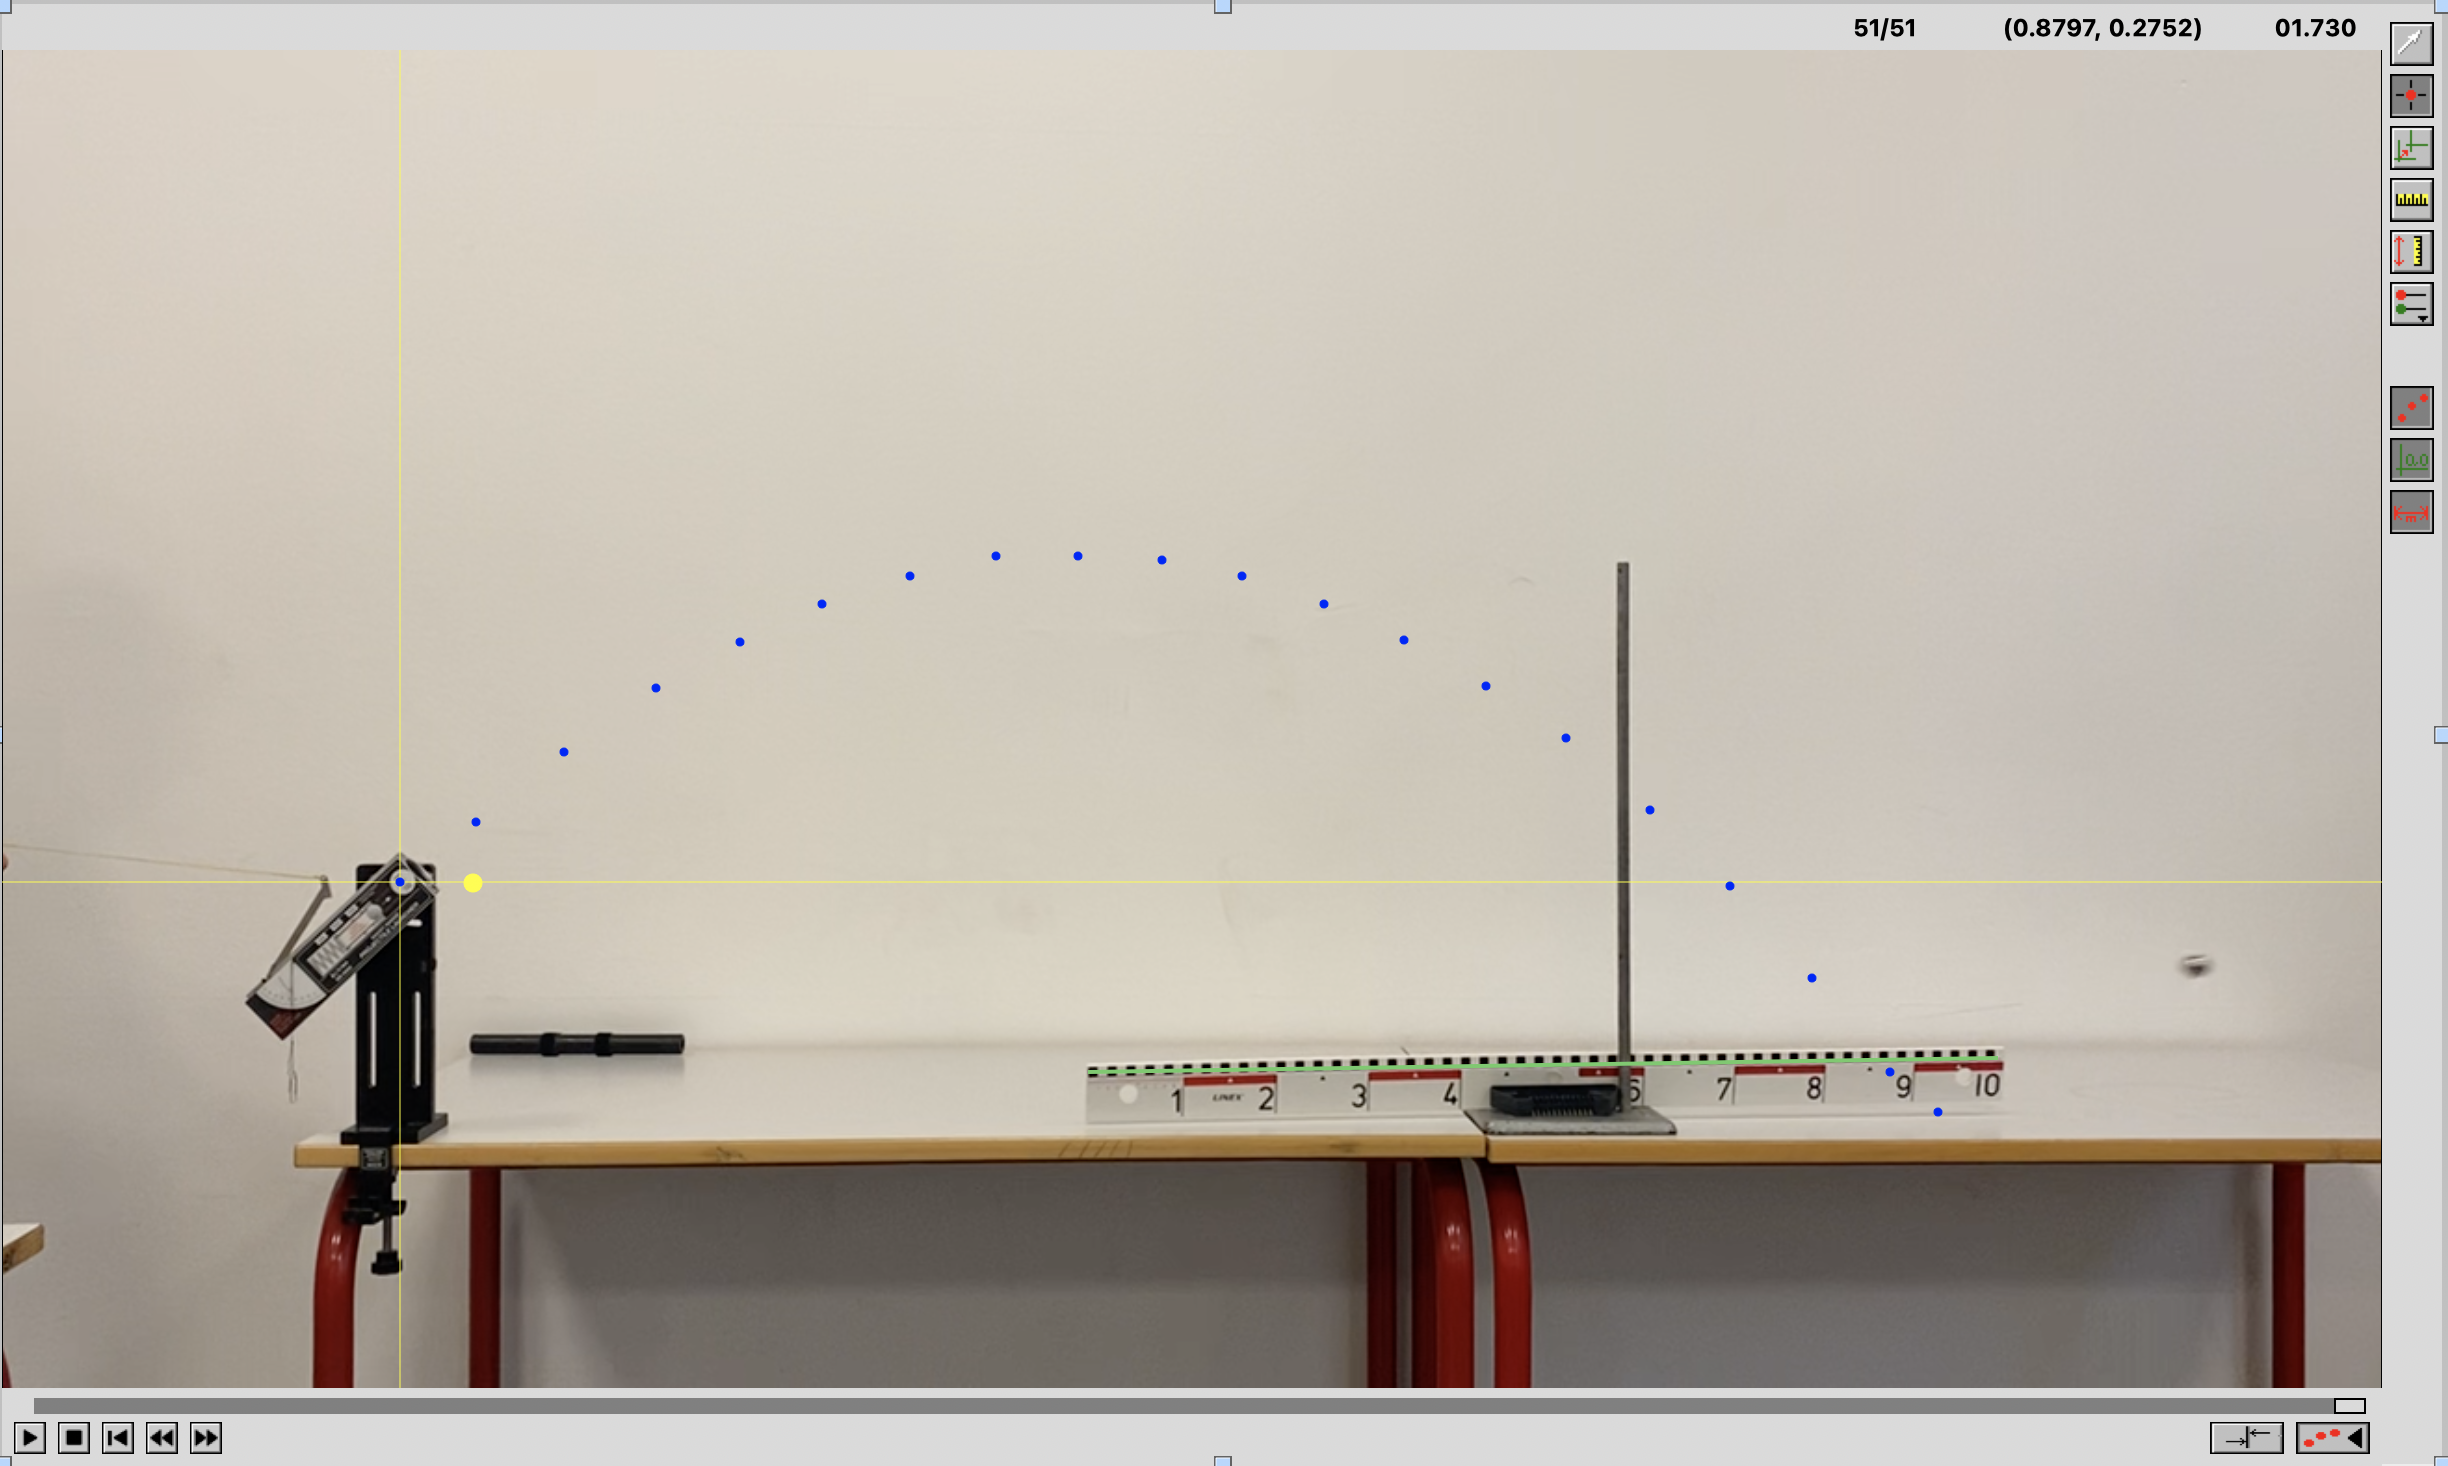
\includegraphics[width=\textwidth]{videotracking45.png}
\end{center}
\caption{Video-tracking lavet i LoggerPro}
\label{fig:tracking}
\end{figure}
Ifølge uafhængighedsprincippet vil den vandrette og lodrette bevægelse foregå uafhængigt af hinanden.
Vi indsætter et koordinatsystem med origo ved kanonmundingen, og kuglen ville, hvis uafhængighedsprincippet holder, være sammensat af to forskellige bevægelser: en horisontalt jævn bevægelse og vertikalt konstant accelereret bevægelse.

Vi undersøger først, om der er en horisontalt jævn bevægelse ved at kigge på $(t,x)$-grafen, der ses i \cref{fig:tx}.
Hvis der er tale om en jævn bevægelse vil punkterne ligge på en ret linje, og hældningen på linjen vil være kuglens vandrette fart.
Det er da også tilfældet, at de tilnærmelsesvist ligger på en ret linje, og fra den lineære regression i Logger Pro fås, at kuglens vandrette fart er 
\[
v_x=2,712 \;\unit{m/s} 
\] 
\begin{figure}[H]
\begin{center}
  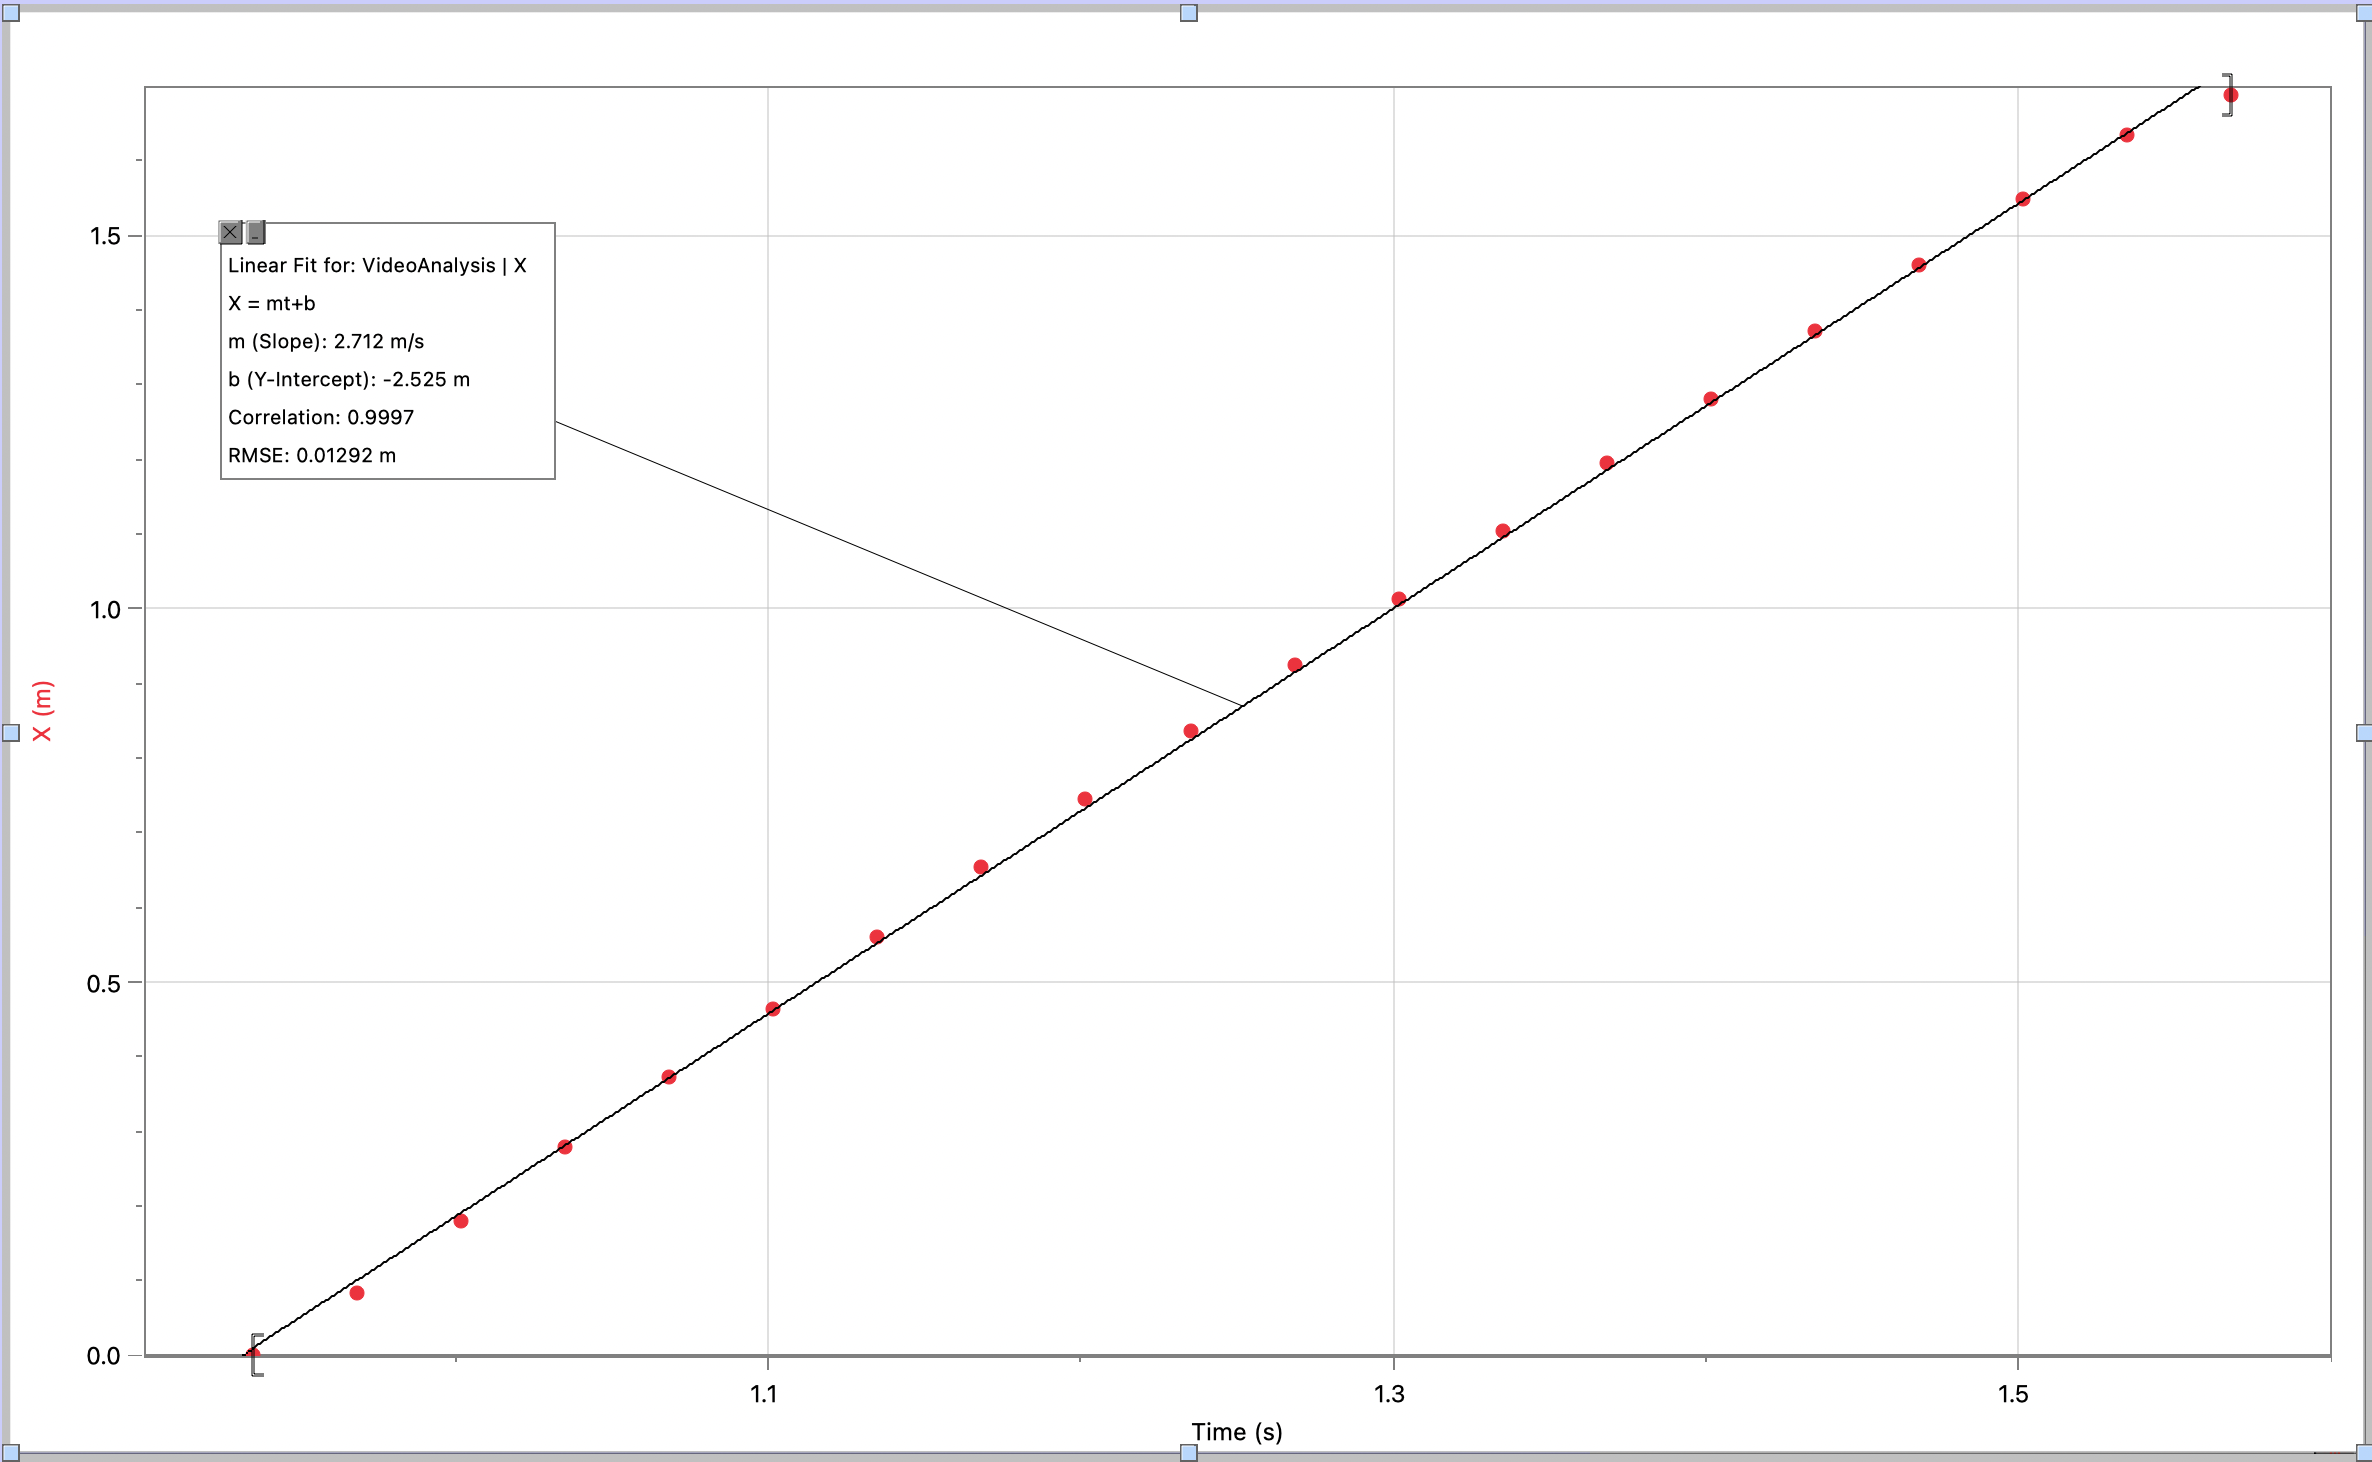
\includegraphics[scale=0.37]{(t,x)45.png}
\end{center}
  \caption{(t,x)-graf for bevægelsen}
  \label{fig:tx}
\end{figure}

Vi ser nu på den vertikale bevægelse.
Hvis der er tale om en jævnt accelereret bevægelse, så må der gælde, at punkterne på $(t,v_y)$-grafen må ligge på en ret linje, hvis hældning er den vertikale bevægelses acceleration.
$(t,v_y)$-grafen ses da i \cref{fig:tv_y}.
\begin{figure}[H]
\begin{center}
  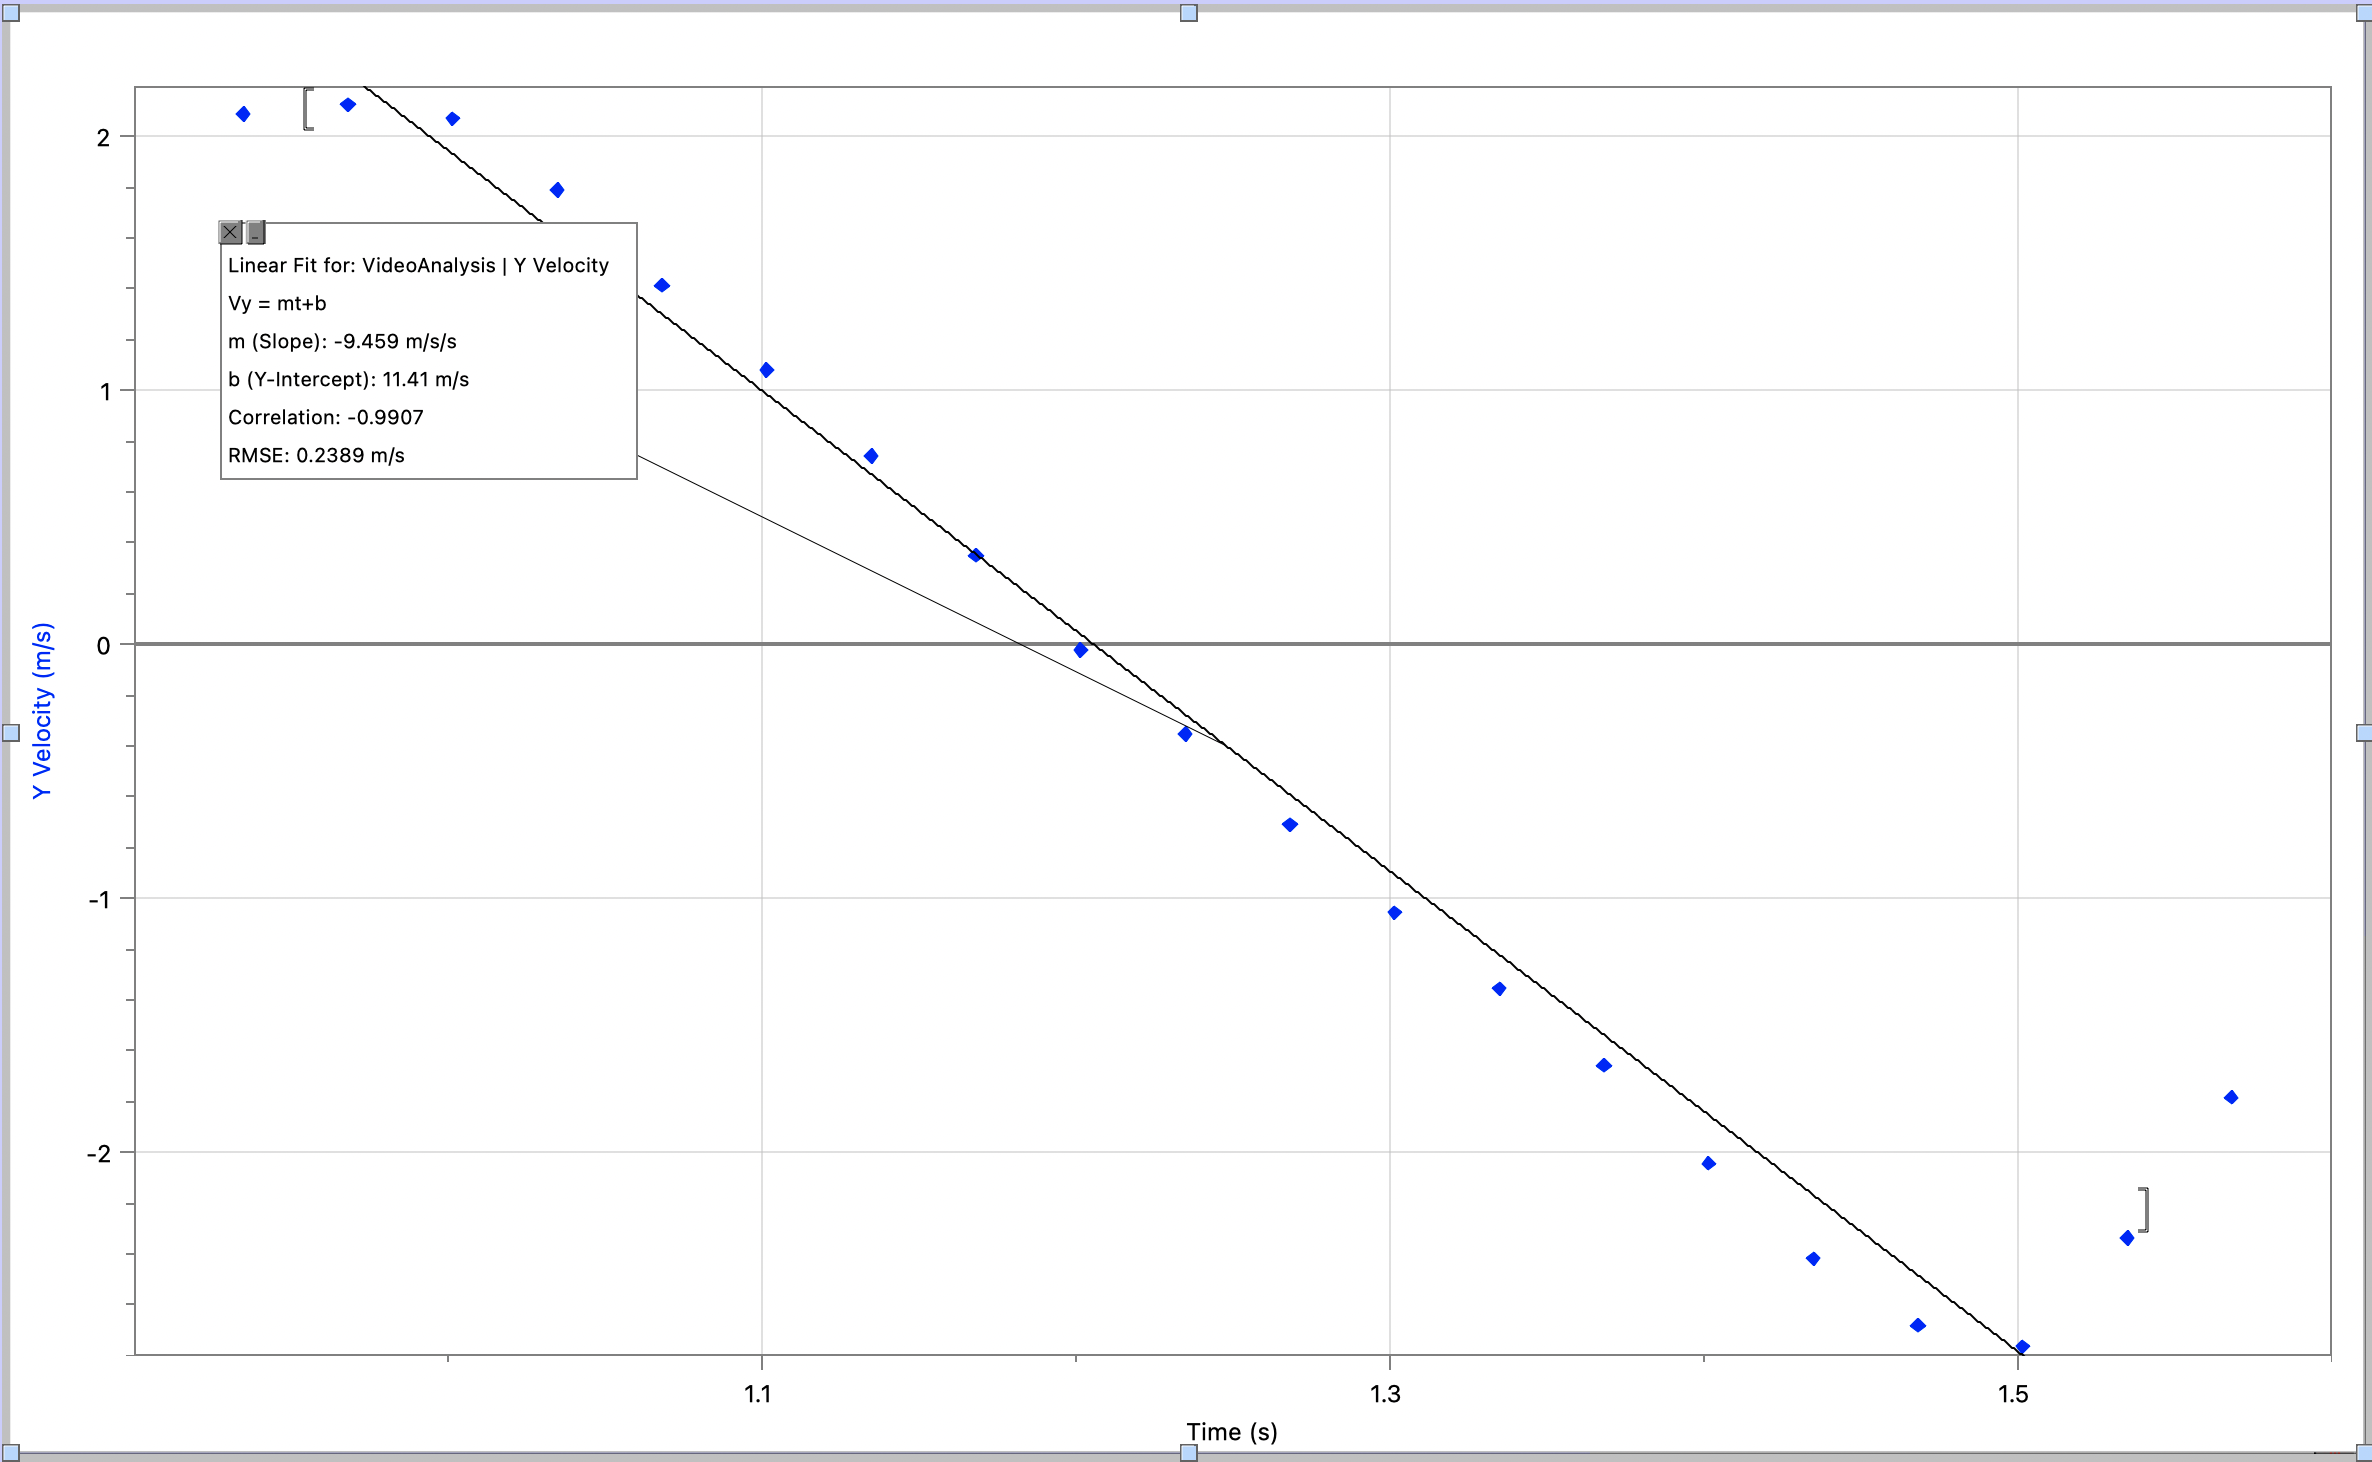
\includegraphics[scale=0.37]{(t,v_y)45.png}
\end{center}
  \caption{$(t,v_y)$-graf for bevægelsen}
\label{fig:tv_y}
\end{figure}
Punkterne ligger tilnærmelsesvist på en ret linje, og en lineær regression laves, dog uden det første og sidst punkt, da kuglen ikke er helt ude af kanonen i det første punkt og bolden rammer bordet i det sidste.
Fra regressionen har vi, at accelerationen på den vertikale bevægelse er 
\[
a_y=-9,459
\] 
Dette er meget tæt på den teoretiske værdi, der er tyngdeaccelerationen $g$.

Vi har nu set, at det skrå kast er sammensat af to bevægelser: en horisontalt jævn bevægelse og vertikalt konstant accelereret bevægelse.
Altså gælder uafhængighedsprincippet.

En konsekvens af, at det skrå kast er sammensat af en horisontalt jævn bevægelse og vertikalt konstant accelereret bevægelse er, at banekurven må være en parabel.
Dette fremgår af $(x,y)$-grafen, der ses i \cref{fig:xy}.
\begin{figure}[H]
\begin{center}
  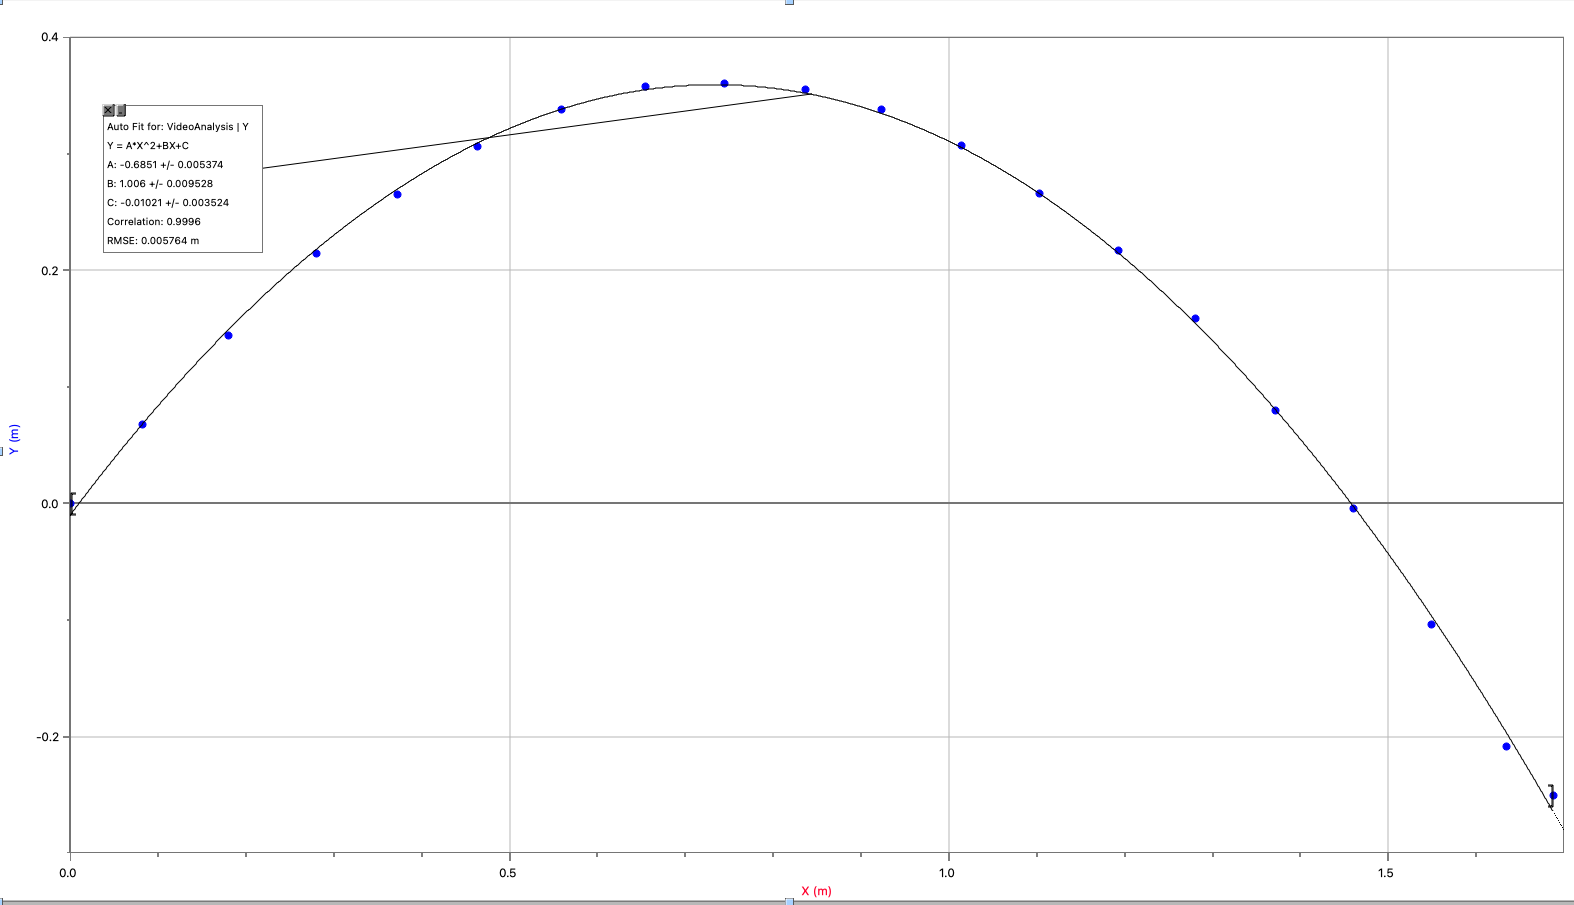
\includegraphics[width=\textwidth]{(x,y)45.png}
\end{center}
  \caption{(x,y)-grafen for bevægelsen}
\label{fig:xy}
\end{figure}
Vi vil nu undersøge henholdsvis kastevidden $x_{\text{max} }$ og stighøjden $y_{\text{max} }$ som funktion af elevationsvinklen.
De målte data for sammenhængen mellem elevationsvinklen og $x _{\text{max} }$ samt $y_{\text{max} }$ målt ved en bestemt startfart $v_0$ ses i \cref{fig:tabel}, hvor $v_0$ er målt ved det lodrette kast.
Da kanonen er ladet til det samme hak, må alle forsøgene have samme $v_0$.
\begin{figure}[H]
\begin{center}
  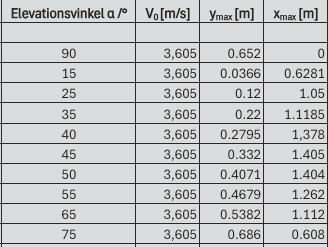
\includegraphics[scale=0.5]{tabel.png}
\end{center}
  \caption{Sammenhæng mellem elevationsvinklen og $x _{\text{max} }$ samt $y_{\text{max} }$ målt ved bestemt $v_0$ }
\label{fig:tabel}
\end{figure}
Teoretisk gælder der for $y_{\text{max} }$, at
\begin{equation}
  \label{eq:y_max}
\begin{split}
  y _{\text{max} }&=\frac{v_0^2 \cdot \sin^2\left(\alpha\right) }{2 \cdot g}\\
  &=\frac{\left(3,605 \;\unit{m/s} \right)^2 \cdot \sin^2\left(\alpha\right) }{2 \cdot 9,82 \;\unit{m/s^2} }
\end{split}
\end{equation}
De målte punkter ses ift. de teoretisk udregnede værdier med ligning \ref{eq:y_max} i GeoGebra ses i \cref{fig:y_max}, hvor elevationsvinklen i grader er ad $x$-aksen og $y_{\text{max} }$ i meter er op ad $y$-aksen. 
Det ses, at punkterne ligger tilnærmelsesvist på grafen.
\begin{figure}[H]
\begin{center}
  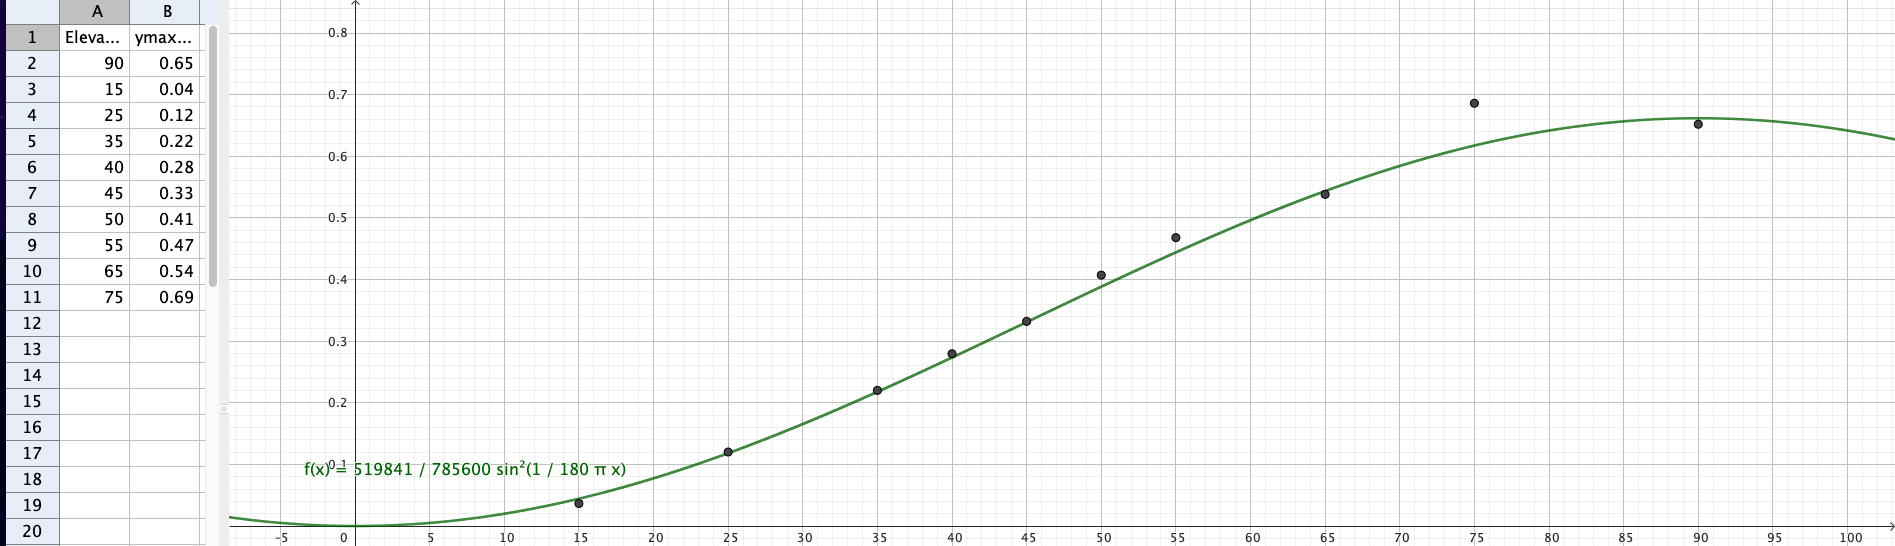
\includegraphics[width=\textwidth]{y_max.png}
\end{center}
  \caption{De målte punkter ift. de teoretisk udregnede værdier for $y_{\text{max} }$}
\label{fig:y_max}
\end{figure}
Vi vil nu undersøge, hvordan $x_{\text{max} }$ afhænger af elevationsvinklen $\alpha$. 
Teoretisk gælder der for $x_{\text{max} }$, at
\begin{equation}
  \label{eq:x_max}
\begin{split}
  x _{\text{max} }&=\frac{v_0^2 \cdot \sin\left(2 \cdot \alpha\right) }{g}\\
  &=\frac{\left(3,605 \;\unit{m/s} \right)^2 \cdot \sin\left(2 \cdot \alpha\right) }{9,82 \;\unit{m/s^2} }
\end{split}
\end{equation}
De målte punkter ses ift. de teoretisk udregnede værdier med ligning \ref{eq:x_max} i GeoGebra ses i \cref{fig:x_max}, hvor elevationsvinklen i grader er ad $x$-aksen og $x_{\text{max} }$ i meter er op ad $y$-aksen.
Det ses, at punkterne ligger tilnærmelsesvist på grafen.
\begin{figure}[H]
\begin{center}
  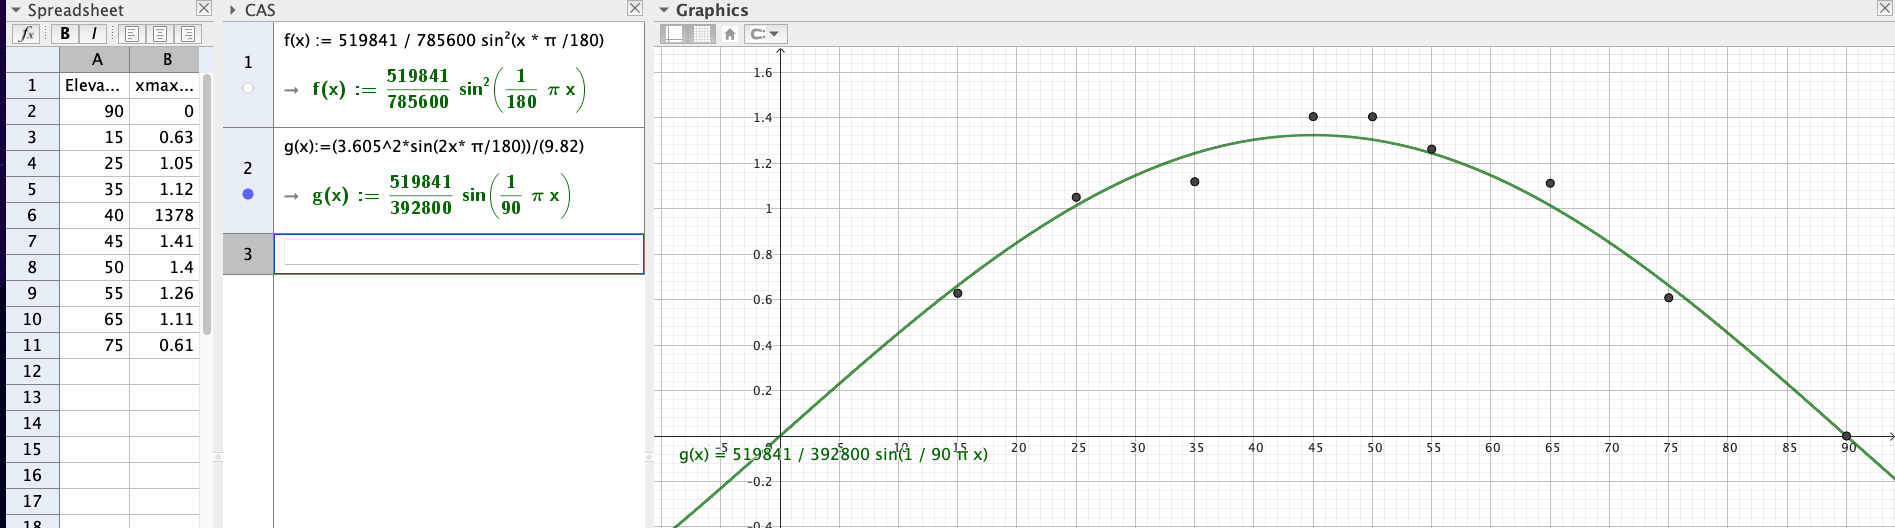
\includegraphics[width=\textwidth]{x_max.png}
\end{center}
\caption{De målte punkter ift. de teoretisk udregnede værdier for $x_{\text{max} }$}
\label{fig:x_max}
\end{figure}

\section*{Fejlkilder}
Eventuelle parallakse-problemer ved filmningen vil have indflydelse på de yderste målinger (tæt på siderne af videoen).

\section*{Konklusion}
Vi har set, at uafhængighedsprincippet gælder for den undersøgte bevægelse, der er sammensat af en horisontalt jævn bevægelse og vertikalt konstant accelereret bevægelse.
En konsekvens af dette er, at banekurven er en parabel.
Til sidst har vi undersøgt kastevidden $x_{\text{max} }$ og stighøjden $y_{\text{max} }$ som funktion af elevationsvinklen $\alpha$, hvor de målte værdier passer nogenlunde med de teoretiske værdier. 


\end{document}
